\begin{figure}
    \centering
    \begin{subfigure}{0.45\linewidth}
        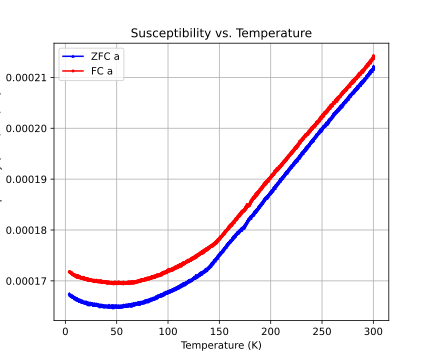
\includegraphics[width=\linewidth]{pdf_files/MvsT_a.pdf}
        \caption{M vs. T for the a-axis. FC-ZFC splitting is observed with FC displaying a higher susceptibility.}
        \label{fig:MvsT_a}
    \end{subfigure}
    \begin{subfigure}{0.45\linewidth}
        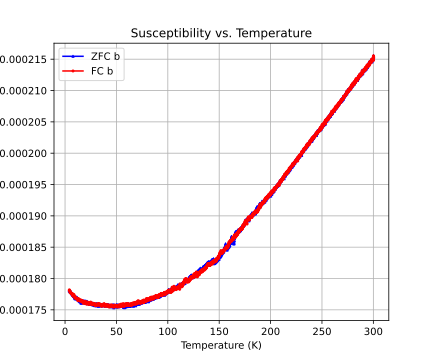
\includegraphics[width=\linewidth]{pdf_files/MvsT_b.pdf}
        \caption{M vs. T for the b-axis. No FC-ZFC splitting can be observed as any difference is within the error of measurement.}
        \label{fig:MvsT_b}
    \end{subfigure}
    \begin{subfigure}{0.45\linewidth}
        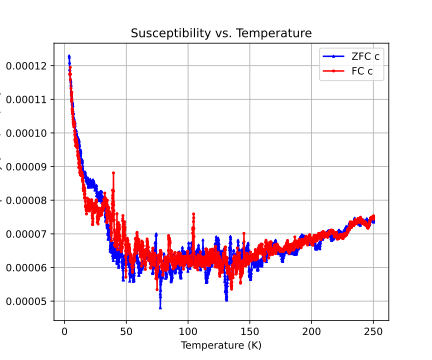
\includegraphics[width=\linewidth]{pdf_files/MvsT_c.pdf}
        \caption{M vs. T for the c-axis. Data very noisy due to thinness of sample in this orientation.}
        \label{fig:MvsT_c}
    \end{subfigure}
    
    \caption{M vs. T measurements for 3 different orientations, denoted a-axis, b-axis and c-axis respectively. The x-axes show the temperature measured in Kelvin, the y-axes the volume susceptibility measured in emu/cm³/Oe.}
    \label{fig:MvsT-tot}
\end{figure}